\documentclass[main.tex]{subfiles}

\begin{document}

\chapter{Examined systems}\label{ch:examined_systems}

\section{Silicon}\label{sec:systems_silicon}

Silicon is the fundamental material in integrated circuits and as such is one of the pillars of the digital revolution.
Analogue to the Stone, Bronze or Iron Age, this age of civilization can thus be called the Silicon Age \cite{chabal_fundamental_2001}.
Consequently, silicon is a well studied material from an experimental and theoretical standpoint with established properties.
This combined with the fact that \acrshort{dft} calculations on silicon are not particularly expensive makes it an ideal system for an introduction to \acrshort{dft} calculation as well as a good benchmarking system.
Consequently, all benchmarks in this thesis were run on silicon first and with the information gained from that, benchmarks on a more expensive system were run.

%Silicon crystallizes in a 

%\begin{figure}[ht!]
%    \centering
%    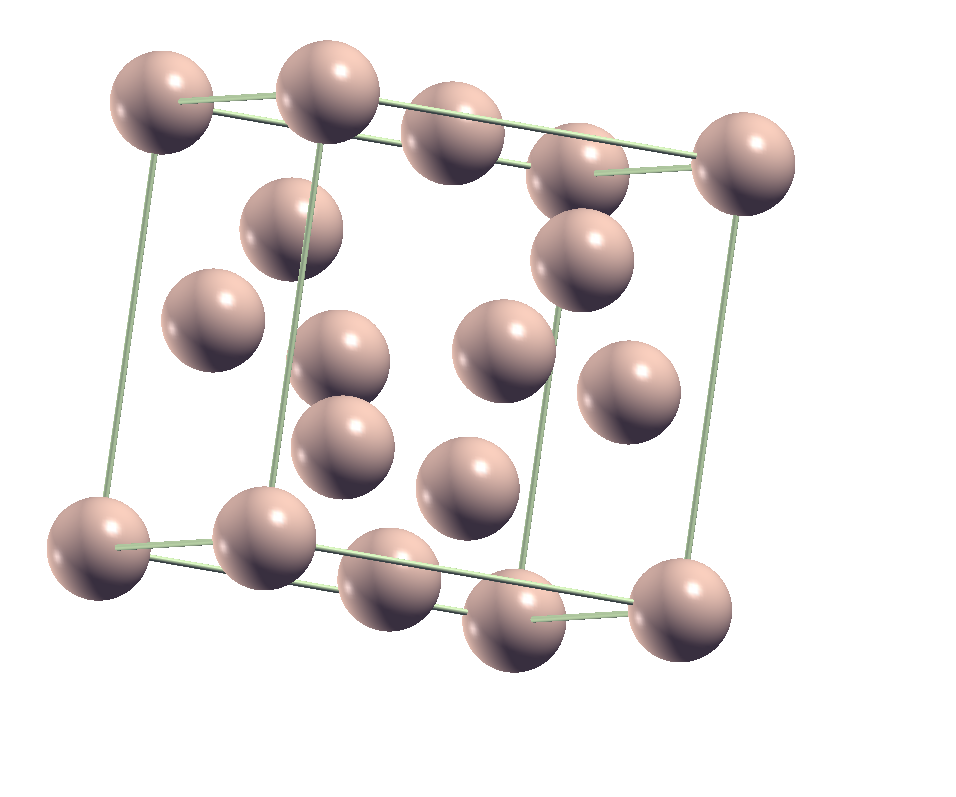
\includegraphics[width=0.5\textwidth]{structure_images/Silicon.png}
%    \caption{Crystal structure of silicon, visualized using XCrySDen \cite{kokalj_xcrysdennew_1999}}
%\end{figure}

\subsection{Computational parameters}

The calculations in ch. \ref{ch:optimisation_scf} and \ref{ch:optimization_ph} were made with a plane wave cutoff of \(\SI{70}{\rydberg}\) and on a \(40\times40\times40\)/\(6\times6\times6\) k point grid respectively.
All calculations use a PBE (Perdew-Burke-Ernzerhof \cite{perdew_generalized_1996}) XC-functional with a norm-conserving \acrshort{pp} generated using Vanderbilt's method \cite{hamann_erratum_2017}.

\section{\TaS}\label{sec:systems_tas2}

Tantal Disulfide (\TaS) belongs to the class of \acrfull{tmdc}'s

, the most common stoichiometry of which is MX\textsubscript{2}, where M is a transition-metal and X is a chalcogen atom.

\acrshort{tmdc}'s were known and studied as a bulk material since more than five decades \cite{wilson_transition_1969}.
The more recent possibility to do experiments on freestanding monolayers \cite{novoselov_two-dimensional_2005} has brought these materials back into focus, as they show 

Both bulk and monolayer \TaS show superconductivity, with the dimensionality reduction enhancing the critical temperature from \(\SI{0.5}{\kelvin}\) to \(\SI{2.2}{\kelvin}\) \cite{navarro-moratalla_enhanced_2016}.

\subsection{Charge-density waves}

\begin{figure}[ht!]
    \centering
    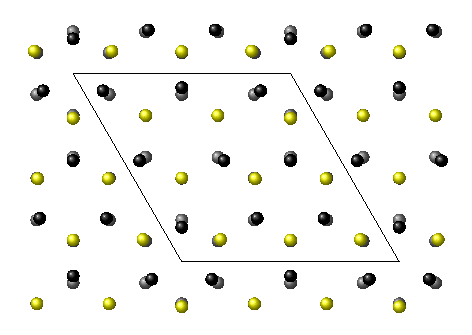
\includegraphics[width=0.5\textwidth]{symmetric.pdf}
    \caption{CAPTION}
\end{figure}

% description inspired by Jan
% cite bulk paper and 2019 2d paper


\subsection{Computational parameters}

All calculations on \TaS were made with a plane wave cutoff of \(\SI{100}{\rydberg}\) and on a \(12\times12\) k point grid.
The calculations use a PBE XC-functional with a norm-conserving \acrshort{pp} generated by Hartwigsen et al. \cite{hartwigsen_relativistic_1998}.
Input files for both the symmetric and charge density wave phase were kindly provided by Dr.\,Jan Berges.

\end{document}
